
\documentclass[12pt,a4paper]{article}
\usepackage[utf8]{inputenc}
\usepackage[english,russian]{babel}
\usepackage{indentfirst}
\usepackage{misccorr}
\usepackage{graphicx}
\usepackage{amsmath}

\graphicspath{{pictures/}}
\DeclareGraphicsExtensions{.pdf,.png,.jpg, .mps, }


\begin{document}






Дадим альтернативное решение задачи $2$ :\\



{\bf Задача 2 }\\Найти минимальное значение функции $$g(x_1, \ldots, x_N)= \sum \limits_{i=1}^{n} x_i^2 $$ при условии, что 
$$\sum \limits_{i=1}^{n} \frac{1}{\sqrt \omega_i} x_i = C - \sum \limits_{i=1}^{n} a_i $$.\\

Заметим, что наборы чисел $X=(x_1, \ldots, x_N)$ и $Y=(\frac{1}{\sqrt {\omega_1} }, \ldots, \frac{1}{\sqrt {\omega_N}} )$ можно понимать как  $N$-мерные евклидовы векторы в пространстве $R^N$. Соответственно, левая часть  последнего равенства есть скалярное произведение X и Y, а функция $g(x_1, \ldots, x_N)$ есть $||X||^2$, где $$||X||= \sqrt{x_1^2+
\ldots+x_N^2}$$ - это длина вектора X.\\

То есть наша задача заключается в том, чтобы  минимизировать квадрат длины вектора $X, $ удовлетворяющего условию 
$\sum \limits_{i=1}^{n} \frac{1}{\sqrt \omega_i} x_i = C - \sum \limits_{i=1}^{n} a_i $. Но заметим, что данное условие означает, что вектор $X$ принадлежит гиперплоскости с нормалью $Y=(\frac{1}{\sqrt {\omega_1} }, \ldots, \frac{1}{\sqrt {\omega_N}} )$ .\\

Последнее утверждение требует некоторых пояснений. Как известно, гиперплоскость- это линейная поверхность коразмерности один, то есть линейная оболочка $ n-1 $вектора.  Из линейной алгебры известно, что линейные пространства можно задавать системами линейных уравнений, причем если система имеет ранг $ k$, то задаваемое ей пространство будет иметь размерность $n-k$.  (это доказано на стр. 4  книги Шурыгина В.В, "Аналитическая геометрия, часть 3" ). В нашем случае размерность пространства равна $n-1$, поэтому для задания  гиперплоскости в $n$-мерном пространстве  требуется всего одно уравнение. Запишем его в виде $a_1x_1 + \dots + a_nx_n=c$. Согласно общей теории, это уравнение задает плоскость размерности n-1. Но с другой стороны, это уравнение можно переписать в виде  $ <a,x> =c$, то есть вектор a перпендикулярен всем векторам x из этой гиперплоскости.  То есть a - вектор нормали к данной гиперплоскости.\\

Данное утверждение, сформулированное как  " в ортонормированной  системе координат главный вектор плоскости является и нормальным ее вектором" доказано на стр. 99  учебника A.E.Умнова "Аналитическая геометрия и линейная алгебра", Москва, МФТИ, 2011.\\


Из курса линейной алгебры известно, что минимизирует расстояние от точки до гиперплоскости - перпендикуляр, опущенный из этой точки на гиперплоскость (это непосредственно следует из многомерной  теоремы Пифагора).\\
 Но перпендикуляр - это вектор, параллельный нормали к поверхности, а  выше мы уже пояснили, что нормаль к  нашей гиперплоскости - это вектор $Y$.\\

$\Rightarrow X=tY,$ то есть $(x_1, \dots, x_n) = t(\frac{1}{\sqrt {\omega_1} }, \ldots, \frac{1}{\sqrt {\omega_N}} )$\\

Подставим выражение для X в условие  $(X,Y) = C- \sum \limits_{i=1}^{n} a_i $\\

Получим $t||Y||^2 = C -  \sum \limits_{i=1}^{n} a_i $\\



$ \Rightarrow  t^* =   \frac{ C-\sum\limits_{i=1}^{n} a_i} { ||Y||^2} = \frac{ C-\sum\limits_{i=1}^{n} a_i} {\sum\limits_{i=1}^{N} \frac{1}{\omega_i}}$, 


$\Rightarrow min  ||X||^2 =  t^2 ||Y||^2 = t(t||Y||^2) = t(C - \sum \limits_{i=1}^{n} a_i ) =  \frac{ (C-\sum\limits_{i=1}^{n} a_i )^2} {\sum\limits_{i=1}^{N} \frac{1}{\omega_i}}$


$\Rightarrow D_{min}= \sum \limits_{i=1}^{N} \omega_i Var\xi_i  +  \frac{(C-\sum\limits_{j=1}^{N} a_j)^2}
{\sum\limits_{j=1}^{N} \frac{1}{\omega_j}} $


 \begin{figure}[h]
\center{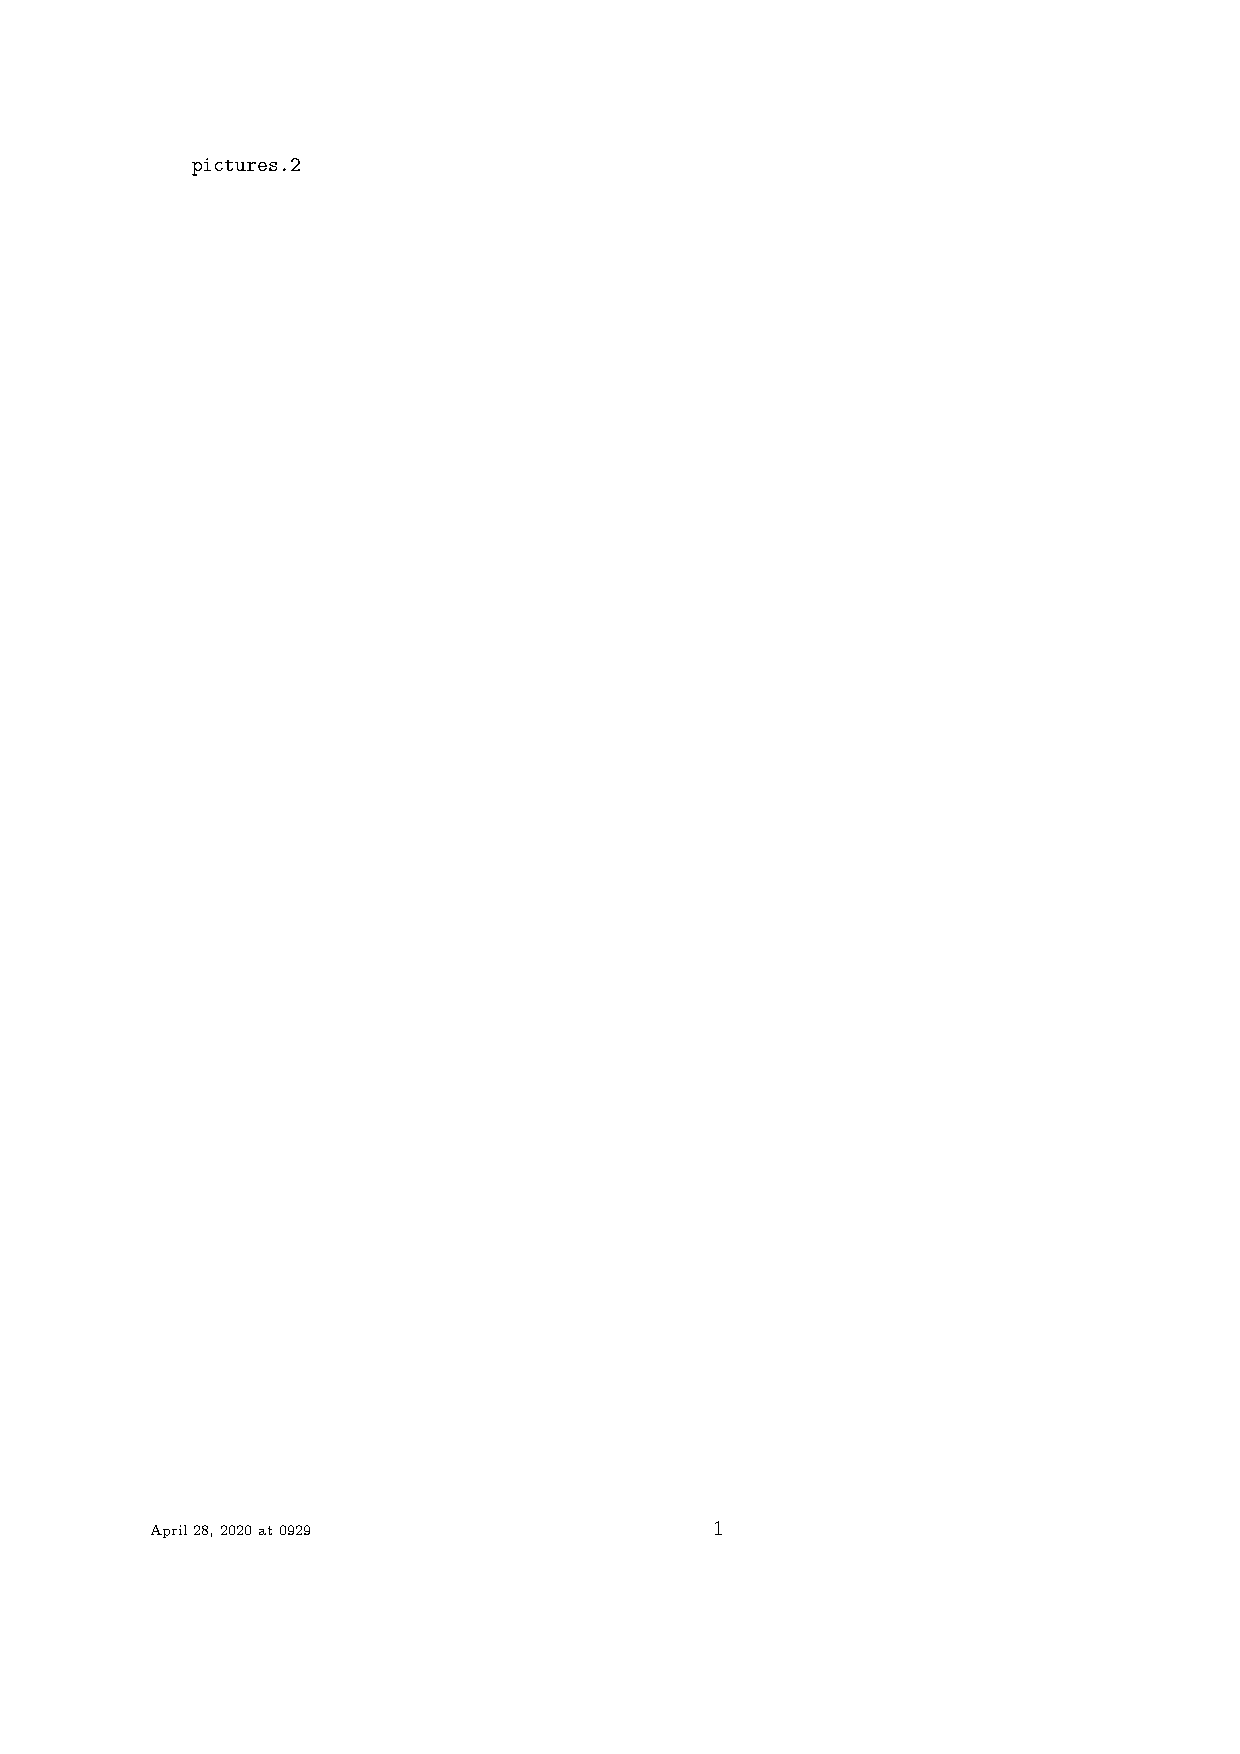
\includegraphics[scale=0.5]{mproof.pdf}}
\caption{ Иллюстрация}
\label{fig:image}
\end{figure}





\end{document}
